\documentclass[11pt]{article}
\usepackage[margin=1in]{geometry}
\usepackage{siunitx}
\usepackage[version=4]{mhchem}
\usepackage{xltabular}
\usepackage{ragged2e}
\usepackage[font=small, skip=3pt, labelfont=bf]{caption}
\usepackage{float}
\usepackage{amsmath}
\usepackage{multirow}
\usepackage{enumitem}
\usepackage{titling}
\usepackage{graphicx}

\DeclareSIUnit{\mpl}{\mol\per\litre}
\DeclareSIUnit{\mmol}{\milli\mol}
\DeclareSIUnit{\gpm}{\gram\per\mol}
\DeclareSIUnit{\ml}{\milli\litre}

\setlist{nosep}

\sisetup{
	space-before-unit = true,
	free-standing-units = true,
	use-xspace = true
}

\title{The Relationship Between the Time Spent Boiling Tap Water and the Remaining Concentration of Dissolved Chlorine}
\author{jjr117}
\date{}

\begin{document}

\begin{titlingpage}
	\maketitle
\end{titlingpage}

\noindent\textbf{Research Question:} How does the time tap water is boiled for affect the amount of remaining concentration of dissolved chlorine in the water?

\section{Introduction}

Chlorine plays a crucial role in modern water treatment systems. The concentration of chlorine in our tap water is too low to harm us, but high enough to kill any deadly bacteria and organisms that were present in the original waste water.

However, while the low concentration of chlorine in tap water makes it safe to consume, it also produces an unpleasant taste. One way my family has been removing the chlorine in tap water is by boiling it before consuming it. However, different sources provide different recommendations on how long water should be boiled for to remove a significant amount of chlorine from the water: from as short as 10 minutes to as long as 20 minutes. Thus, in my experiment, I plan to investigate the relationship between the time spent boiling tap water and the remaining chlorine concentration, and hopefully determine an optimal amount of time water should be boiled for in order to remove a significant amount of chlorine from the water.

\section{Background Information}

Chlorine gas (\ce{Cl2_{(g)}}) is frequently used at water treatment facilities to remove harmful organisms from waste water to produce water which is safe for us to consume. When chlorine gas added to water, the chlorine reacts with water to form hypochlorous acid (\ce{HOCl}):

\centerline{\ce{Cl2_{(g)} + H2O_{(l)} -> HOCl_{(aq)} + H^{+}_{(aq)} + Cl^{-}_{(aq)}}}

Hypochlorous acid is effective at inactivating deadly microbiological organisms like salmonella and E. coli, as well as many viruses. It is able to kill these harmful organisms by disrupting their cell membranes and destroying their protein structures. Thus, through the use of chlorine, water treatment facilities are able to prevent illnesses and death from otherwise infected water.

However, it is not sufficient to add just enough chlorine to disinfect water at the treatment plants. An adequate concentration of chlorine must be sustained throughout the entire distribution system. Otherwise, the water could possibly become infected in intermediate sources and become unsafe to drink by the time it reaches our homes. Because of these concerns, water treatment plants add excess chlorine to treat water such that the water that comes out of the tap still contains a small concentration of free chlorine, or chlorine that has not yet reacted with undesired substances in the water.

The free chlorine in tap water is what causes it to sometimes have an unpleasant taste, even in low concentrations. To remove this excess chlorine, my family boils tap water for around 15 to 20 minutes. Boiling is effective at removing chlorine because the solubility of gases in liquids decreases with increasing temperature, and chlorine is a gas at room temperature. Thus, as the water is heated up, it cannot hold as much free chlorine in the water, and so the free chlorine is released in the form of chlorine gas.

\begin{figure}[H]
	\centering
	\caption{Solubility curve for chlorine: the hotter the water is, the less dissolved chlorine the water can hold.}
	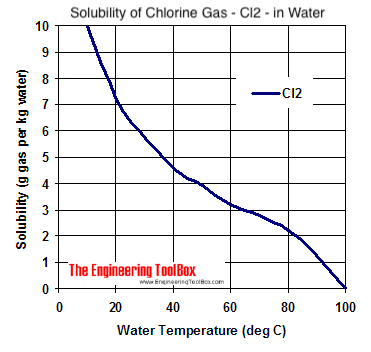
\includegraphics[width=0.5\linewidth]{assets/cl-solubility.png}
\end{figure}

The above solubility curve for chlorine gas in water highlights that a limitation to removing chlorine by boiling water. The solubility of chlorine gas in water is non-zero up until 100 degrees Celsius--the temperature at which water evaporates and no more liquid water left for use. Thus, when the water is at any temperature less than 100 degrees Celsius, some chlorine will still remain in the water. While this limitation is acceptable for use cases like consumption, it may not be sufficient for other use cases like the need for pure water in a lab environment.

Thus, in this experiment, the approach of boiling to remove chlorine from water will also be compared to water deionizers, which are an alternative and established method of filtering out chlorine.

Water deionizers remove chlorine through ion-exchange resins. One resin contains beats contains beads which are positively pre-charged with hydrogen ions (\ce{H^+}), and the other resin contains beads which are negatively pre-charged with hydroxide ions (\ce{OH^-}). Water contaminated with minerals is passed through both resins in the water deionizer. The positively changed resin exchanges its hydrogen ions with cations present in the water, and the negatively changed resin exchanges its hydroxide ions with anions present in the water, such as chloride ions. In the end, the hydrogen ions and hydroxide ions combine to form pure water \ce{H2O}.

% TODO: in-text https://complete-water.com/resources/what-is-deionized-water

\subsection{Hypothesis}
The time spent boiling tap water is inversely proportional to the remaining concentration of dissolved chlorine.

\newpage

\section{Methodology}

To determine the amount of chlorine in a sample of tap water, Mohr's method will be used, which determines the chloride ion concentration in a solution by titrating it with silver nitrate (\ce{AgNO3}) and adding potassium chromate (\ce{K2CrO4}) as an indicator.

Initially, the solution consists of the water sample and a few drops of the potassium chromate indicator, which turns the solution light yellow:

\begin{figure}[H]
	\centering
	\includegraphics[width=0.25\linewidth]{assets/initial.png}
	\caption{Before any silver nitrate solution is added, the colour of the solution is a bright and transparent yellow.}
\end{figure}

As silver nitrate is added to the solution with an unknown concentration of chloride ions, the chloride ions bond with the silver ions to form silver chloride:

\centerline{\ce{Ag^{+}_{(aq)} + Cl^{-}_{(aq)} -> AgCl_{(s)}}}

Since silver chloride is insoluable in water, it produces a white precipitate that can be seen during the titration:

\begin{figure}[H]
	\centering
	\includegraphics[width=0.25\linewidth]{assets/white-precipitate.png}
	\caption{The silver chloride is identified as an unsoluable white precipiate.}
\end{figure}

The titration is complete when the silver ions have reacted with all the chlorine ions in the solution, leaving excess silver ions in the solution. The excess silver ions then react with chromate ions from the potassium chromate indicator to form silver chromate (\ce{Ag2CrO4_{(s)}}):

\centerline{\ce{2Ag^{+}_{(aq)} + CrO4^{2-}_{(aq)} -> Ag2CrO4_{(s)}}}

Silver chromate is a red-brown precipate, and it can be easily identified in the solution as the silver chromate turns the solution from white to a red-brown colour:

\begin{figure}[H]
	\centering
	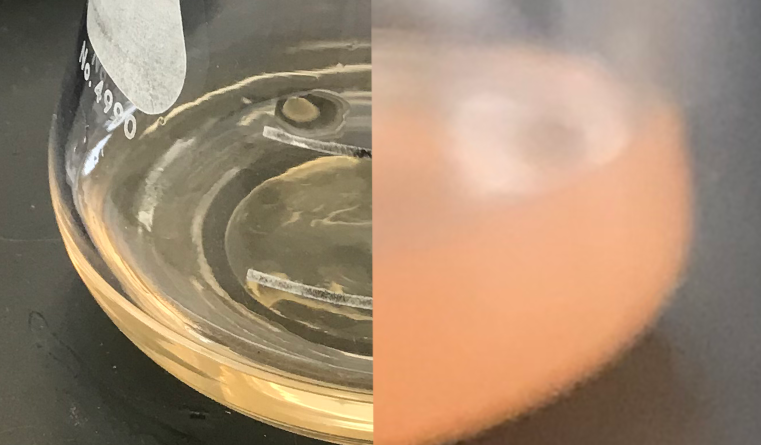
\includegraphics[width=0.3\linewidth]{assets/color-difference}
	\caption{The color difference between the starting point (left image) of the titration and the endpoint of the titration (right image).}
\end{figure}

When the above red-brown colour appears in the solution, it indicates that all the chloride ions have reacted with the silver nitrate and that the titration endpoint has been reached. The amount of titrant (the silver nitrate solution) added is then noted down, and this amount can be used to determine the amount of chloride ions in the water sample.

One potential weakness with Mohr's method is that it is ineffective at determine the chlorine concentration of a sample with other halides, such as iodide or bromide. However, in our situation, tap water % TODO: update

\subsection{Variables}

\textbf{Independent Variable:} Amount of time tap water is boiled

\textbf{Dependent Variable:} Remaining chlorine concentration in water

\begin{table}[H]
	\def\arraystretch{1.5}
	\caption{A list of controlled variables during the experiment.}
	\begin{tabularx}{\linewidth}{|
			>{\RaggedRight}X|
			>{\RaggedRight}X|
			>{\RaggedRight}X|
		}
		\hline
		\textbf{Controlled Variable}
		 & \textbf{Reason for Control}
		 & \textbf{Method of Control}
		\\\hline
		Concentration of Silver Nitrate Solution
		 & The amount of silver nitrate needed to titrate the water samples depends on the concentration used.
		 & 50\ml of silver nitrate solution was prepared beforehand which was enough for all the experiments.
		\\\hline
		Temperature of hot plate
		 & Different temperatures of the hot plate would boil water at different speeds.
		 & The hot plate was kept at the same power level, left on for 15 minutes to reach full power, and then the water samples were boiled sequentially.
		\\\hline
	\end{tabularx}
\end{table}

\subsection{Apparatus}

<?#
I ended up using 2 mL total of 1 mol/L K2CrO4
This produces 0.01M

I remember using 0.01M of AgNO3 as well
?>

\begin{itemize}
	\item 250\ml Erlenmeyer Flask
	\item 250\ml Beaker
	\item 50\ml Burette with 0.1\ml graduations
	\item Burette stand
	\item Hot Plate
	\item 10\ml pipette
	\item Water deionizer (Thermo Scientific HN High Capacity Cartridge.)
	\item 2 $\times$ 100\ml graduated cylinder with 1\ml graduations
	\item 10\ml graduated cylinder
	\item Analytical scale with $\pm$0.0001\gram precision
	\item 1\ml Droppers
\end{itemize}

\subsection{Materials}

\begin{itemize}
	\item Silver Nitrate (\ce{AgNO3_{(s)}}, powdered form)
	\item 0.1 \mpl Potassium Chromate Solution (\ce{K2CrO4_{(aq)}})
	\item Deionized Water
\end{itemize}

\subsection{Procedure}

% TODO: describe initial attempts to create concentrations and how it failed because it was too dilute

Originally, the amount of silver nitrate needed to

\subsection{Risk assessment}

Even though chlorine gas is released when tap water is boiled, the amount of chlorine released is so trace that it poses no appreciable danger. According to toronto.ca, the amount of chlorine in drinking water is regulated to be between 1 and \SI{3}{\mg\per\litre}, which is equal to 1-3 ppm. At this concentration of chlorine gas, mild mucus membrane irritation occurs that can be tolerated for around an hour (<?# todo: https://www.ncbi.nlm.nih.gov/pmc/articles/PMC3136961/ ?>). However, because the experiment is conducted in a large and ventilated room and the chlorine gas from boiling tap water is released over a relatively long period of time, the actual concentration of the chlorine gas at any given moment is much lower, thus posing no threat as a health hazard.

Silver nitrate is hazardous and can stain skin and cause damage if it comes in contact with the eyes. Thus, goggles were worn at all times during the experiment and gloves were worn when handling silver nitrate. In addition, silver nitrate is considered hazardous waste due to its reactivity and toxicity, so it must be disposed properly. After each trial, the solution containing tap water, silver nitrate solution and potassium chromate solution was poured into a temporary beaker for storing waste. Once all the experiments were finished, the remaining silver nitrate solution and the contents of the waste beaker were poured in a hazardous waste container provided by the school, with the concentration of silver nitrate recorded.

In addition, this experiment involves the use of a hot plate at maximum power and boiling water. Thus, it was crucial that the hot plate was placed in an area away from the main titration setup to prevent accidental contact. In addition, gloves were worn when the beakers needed to be added and removed from the hot plate. When the beakers were removed, they were placed on top of cold water in a large 1 liter beaker. This allowed the water to cool down more quickly before it would be used. Theoretically, cooling down the water before titration should not affect the end result, as the purpose of boiling the water is to remove free chlorine dissolved in the water, and when the water is cooled, the free chlorine should have been already released. Once the chlorine gas has been released into the atmosphere, they would not become re-dissolved in the water.

\section{Procedure}

\begin{enumerate}
	\item A silver nitrate solution (\ce{AgNO3(aq)}) was created by measuring out 0.0817\g of solid \ce{AgNO3} and diluting it with 50\ml of deionized water.
	\item A dilute solution of 0.01\mpl \ce{K2CrO4} was created by measuring out 1\ml of the 0.1\mpl \ce{K2CrO4} stock solution and diluting it with 10\ml of deionized water.
	\item The \ce{AgNO3} solution was poured into a burette.
	\item 10\ml of tap water was transported into a 100\ml Erlenmeyer flask using a 10\ml pipette.
	\item Approximately 1\ml of the 0.01\mpl \ce{K2CrO4} solution was added to the 10\ml of tap water using a dropper.
	\item The initial volume of \ce{AgNO3} solution in the burette was noted down. The tap water was titrated with the \ce{AgNO3} solution until the solution turned reddish-brown (see Figure x). The final amount of solution in the burette was noted down.
	\item Steps 4 to 6 were repeated for 2-3 more trials.
	\item Steps 4 to 7 were repeated for deionized water and water boiled for 3, 6, 9, and 20 minutes using a hot plate.
\end{enumerate}

\section{Data}

% \begin{noindent}
<?
const silverNitrateSol = {
	mass: 0.0817,
	volume: 0.05,
	concentration: undefined,
};

/*
[0]: # of minutes boiled (or 'deionized' if the water was deionized)
[1]: mL of AgNO3 needed
[2]: mL of H2O used
*/

const rawData = [
	['deionized', 11.75 - 11.45, 10],
	['deionized', 31.15 - 30.8, 10],
	['deionized', 31.6 - 31.15, 10],
	[0, 11.45 - 10.15, 10],
	[0, 17.45 - 16.2, 10],
	[0, 18.7 - 17.45, 10],
	[3, 5.6 - 4.3, 10],
	[3, 14.3 - 13, 10],
	[3, 13 - 11.75, 10],
	[6, 20.15 - 18.7, 10],
	[6, 30.8 - 29.4, 10],
	[6, 7 - 5.6, 10],
	[9, 16.2 - 14.3, 10],
	[9, 10.15 - 8.65, 10],
	[20, 26.4 - 20.15, 10],
	[20, 29.4 - 26.4, 5],
];

const headers = ['minutesBoiled', 'titrantAmount', 'amountOfWater'];

const data = rawData.map(row => Object.fromEntries(R.zip(headers, row)));
?>
% \end{noindent}

\begin{table}[H]
	\caption{Data collected during the experiment over 16 trials. Note that the amount of water used for Trial 16 is only 5\ml because }
	\def\arraystretch{1.5}
	\begin{tabularx}{\linewidth}{|
			>{\RaggedRight}X|
			>{\RaggedRight}X|
			>{\RaggedRight}X|
			>{\RaggedRight}X|
		}
		\hline
		\textbf{Trial Number}                &
		\textbf{Time Boiled} /\si{\minute}   &
		\textbf{Titrant Amount} /$\pm$0.1\ml &
		\textbf{Amount of Water} /$\pm$0.05\ml
		\\\hline
		% \begin{noindent}
		<? for (const [rowIndex, row] of data.entries()) { ?>
			Trial <?= rowIndex + 1 ?>
			& <?= row.minutesBoiled ?>
			& <?= row.titrantAmount.toFixed(2) ?>
			& <?= row.amountOfWater ?>
			\\\hline
		<? } ?>
		% \end{noindent}
	\end{tabularx}
\end{table}

\section{Calculations}

To determine the concentration of chloride ions in the water, the amount of water and the amount of titrant is used.

The mass of \ce{AgNO3_{(s)}} used to create the silver nitrate solution was <?= silverNitrateSol.mass ?>\g. The analytical scale used to weigh this amount had an uncertainty of $\pm$0.0001\g. Using this information, the number of moles of silver nitrate in the solution can be determined:
%
\begin{align*}
	n_{\ce{AgNO3}} & = \frac{m_{\ce{AgNO3}}}{M_{\ce{AgNO3}}}
	\\
	n_{\ce{AgNO3}} & = \frac{(<?= silverNitrateSol.mass ?> \pm 0.0001)\g}{169.87\gpm}
	\\
	<? silverNitrateSol.moles = silverNitrateSol.mass / 169.87 -?>
	n_{\ce{AgNO3}} & = <?= sf(silverNitrateSol.moles, 3) ?>\mol \pm <?= sf(0.0001 / silverNitrateSol.mass * 100, 1) ?>\%
\end{align*}

The silver nitrate was diluted with 50\ml of deionized water using a graduated cylinder with an uncertainty of 0.5\ml or 1\%. Using the number of moles of \ce{AgNO3} in the solution, the concentration of the solution can be determined:
%
\begin{align*}
	c & = \frac{n}{V}
	\\
	c & = \frac{<?= sf(silverNitrateSol.moles, 3) ?>\mol \pm 0.1\%}{<?= silverNitrateSol.volume ?>\litre \pm 1\%}
	\\
	<? silverNitrateSol.concentration = silverNitrateSol.moles / silverNitrateSol.volume -?>
	c & = <?= sf(silverNitrateSol.concentration, 3) ?>\mpl \pm 1.1\%
\end{align*}

The concentration of the \ce{AgNO3} solution can then be used to determine the moles of \ce{AgNO3} for a given volume of the silver nitrate solution. For example, using the data in Trial 4, the volume of the silver nitrate solution needed to titrate the water was 1.30\ml $\pm$ 0.1\ml, or 1.30\ml $\pm$ 7.7\%, giving the following number of moles of \ce{AgNO3}:
%
\begin{align*}
	n & = V \times c
	\\
	n & = (1.30\ml \pm 7.7\%) \times (<?= sf(silverNitrateSol.concentration, 3) ?>\mpl \pm 1.1\%)
	\\
	<? const trial1Calculations = { molesOfSilverNitrate: silverNitrateSol.concentration * 1.30 } -?>
	n & = <?= sf(trial1Calculations.molesOfSilverNitrate, 3) ?>\mmol \pm 8.8\%
\end{align*}

The number of moles of \ce{AgNO3} can then be used to determine the number of moles of chloride ions in the water. The mole ratio between \ce{Ag^-} and \ce{Cl^-} can be determined from the reaction taking place between the silver nitrate and the chloride ions:

\centerline{\ce{AgNO3_{(aq)} + Cl^{-}_{(aq)} -> AgCl_{(s)} + NO3^{-}_{(aq)}}}

From the above balanced chemical equation, it can be determined that the mole ratio between \ce{Ag^-} and \ce{Cl^-} is 1. Therefore, the number of moles of \ce{AgNO3} is equal to the number of moles of \ce{Cl^-}:
%
\begin{align*}
	n_{\ce{Cl^-}} & = n_{\ce{AgNO3}}
	\\
	<? trial1Calculations.molesOfChlorine = trial1Calculations.molesOfSilverNitrate -?>
	n_{\ce{Cl^-}} & = <?= sf(trial1Calculations.molesOfChlorine, 3) ?>\mmol \pm 8.8\%
\end{align*}

From here, the concentration of chloride ions in the water can be determined knowing that the amount of water used was 10\ml $\pm$ 0.05\ml, or 10\ml $\pm$ 0.5\%:
%
\begin{align*}
	c & = \frac{<?= sf(trial1Calculations.molesOfChlorine, 3) ?>\mmol \pm 8.8\%}{10\mL \pm 0.5\%}
	\\
	c & = <?= sf(trial1Calculations.molesOfChlorine / 10, 3) ?>\mpl \pm 9\%
\end{align*}

The above calculations were performed for each of the values in the 16 trials, producing the following values:

% \begin{noindent}
<?
function calculateMolesOfChlorine(rowIndex: number) {
	const row = data[rowIndex];
	return row.titrantAmount * silverNitrateSol.concentration / row.amountOfWater;
}

function calculateMolesOfChlorineUncertaintyPercentage(rowIndex: number) {
	const row = data[rowIndex];
	const silverNitrateUncertaintyPercentage = 1.1;
	const titrantUncertaintyPercentage = (0.1 / row.titrantAmount) * 100;
	const amountOfWaterUncertaintyPercentage = 0.5;
	const totalUncertaintyPercentage =
		silverNitrateUncertaintyPercentage +
		titrantUncertaintyPercentage +
		amountOfWaterUncertaintyPercentage;
	return totalUncertaintyPercentage;
}

function formatFinalMolesOfChlorine(rowIndex: number) {
	const moles = calculateMolesOfChlorine(rowIndex);
	const uncertaintyPercentage = calculateMolesOfChlorineUncertaintyPercentage(rowIndex);
	return roundToUncertaintyDecimalPlaces(moles, uncertaintyPercentage);
}

function roundToUncertaintyDecimalPlaces(value: number, uncertaintyPercentage: number) {
	const uncertaintyString = sf(value * (uncertaintyPercentage / 100), 1);
	const decimalPlaces = uncertaintyString.length - uncertaintyString.indexOf('.') - 1;
	return `${value.toFixed(decimalPlaces)} $\\pm$ ${uncertaintyString}`;
}
?>
% \end{noindent}

\begin{table}[H]
	\caption{The concentration of chloride ions in each trial obtained from performing the above calculations. For each variation of boiling time, the uncertainty in the average concentration of \ce{Cl^-} was determined by taking the average of the uncertainties for each individual trial.}
	\def\arraystretch{1.5}
	\begin{tabularx}{\linewidth}{|
			>{\RaggedRight}X|
			>{\RaggedRight}X|
			>{\RaggedRight}X|
		}
		\hline
		\textbf{Time Boiled} /\si{\minute}
		 & \textbf{Concentration of \ce{Cl^-}} /\si{\mpl}
		 & \textbf{Average concentration of \ce{Cl^-}} /\si{\mpl}
		\\\hline
		% \begin{noindent}
		<? for (const [rowIndex, row] of data.entries()) { ?>
			<?= row.minutesBoiled ?>
			& <?= formatFinalMolesOfChlorine(rowIndex) ?>
			&
			<? if (row.minutesBoiled !== data[rowIndex - 1]?.minutesBoiled) { ?>
				<?
					const end = data.findIndex((dataRow, i) => i >= rowIndex && dataRow.minutesBoiled !== row.minutesBoiled);
					const trialIndexes = R.range(rowIndex, end === -1 ? data.length : end);
					const trialMoles = trialIndexes.map(
						(trialIndex) => calculateMolesOfChlorine(trialIndex)
					);
					const averageMolesOfChlorine = R.mean(trialMoles);
					const sumOfUncertaintyOfAverage = R.sum(trialIndexes.map(
						(trialIndex) =>
							calculateMolesOfChlorine(trialIndex) *
							(calculateMolesOfChlorineUncertaintyPercentage(trialIndex) / 100)
					));
					const uncertaintyPercentageOfAverage =
						sumOfUncertaintyOfAverage / R.sum(trialMoles) * 100
				?>
				\multirow{
					<?=
						R.count(
							(r) => r.minutesBoiled === row.minutesBoiled,
							data
						)
					?>
				}{*}{<?= roundToUncertaintyDecimalPlaces(averageMolesOfChlorine, uncertaintyPercentageOfAverage) ?>}
				\\\cline{1-2}
			<? } else if (row.minutesBoiled !== data[rowIndex + 1]?.minutesBoiled) { ?>
				\\\hline
			<? } else { ?>
				\\\cline{1-2}
			<? } ?>
		<? } ?>
		% \end{noindent}
	\end{tabularx}
\end{table}

\newpage

Plotting these values on a graph yields the following result:

\begin{figure}[H]
	\centering
	\caption{The concentration of chlorine remaining plotted against boiling time.}
	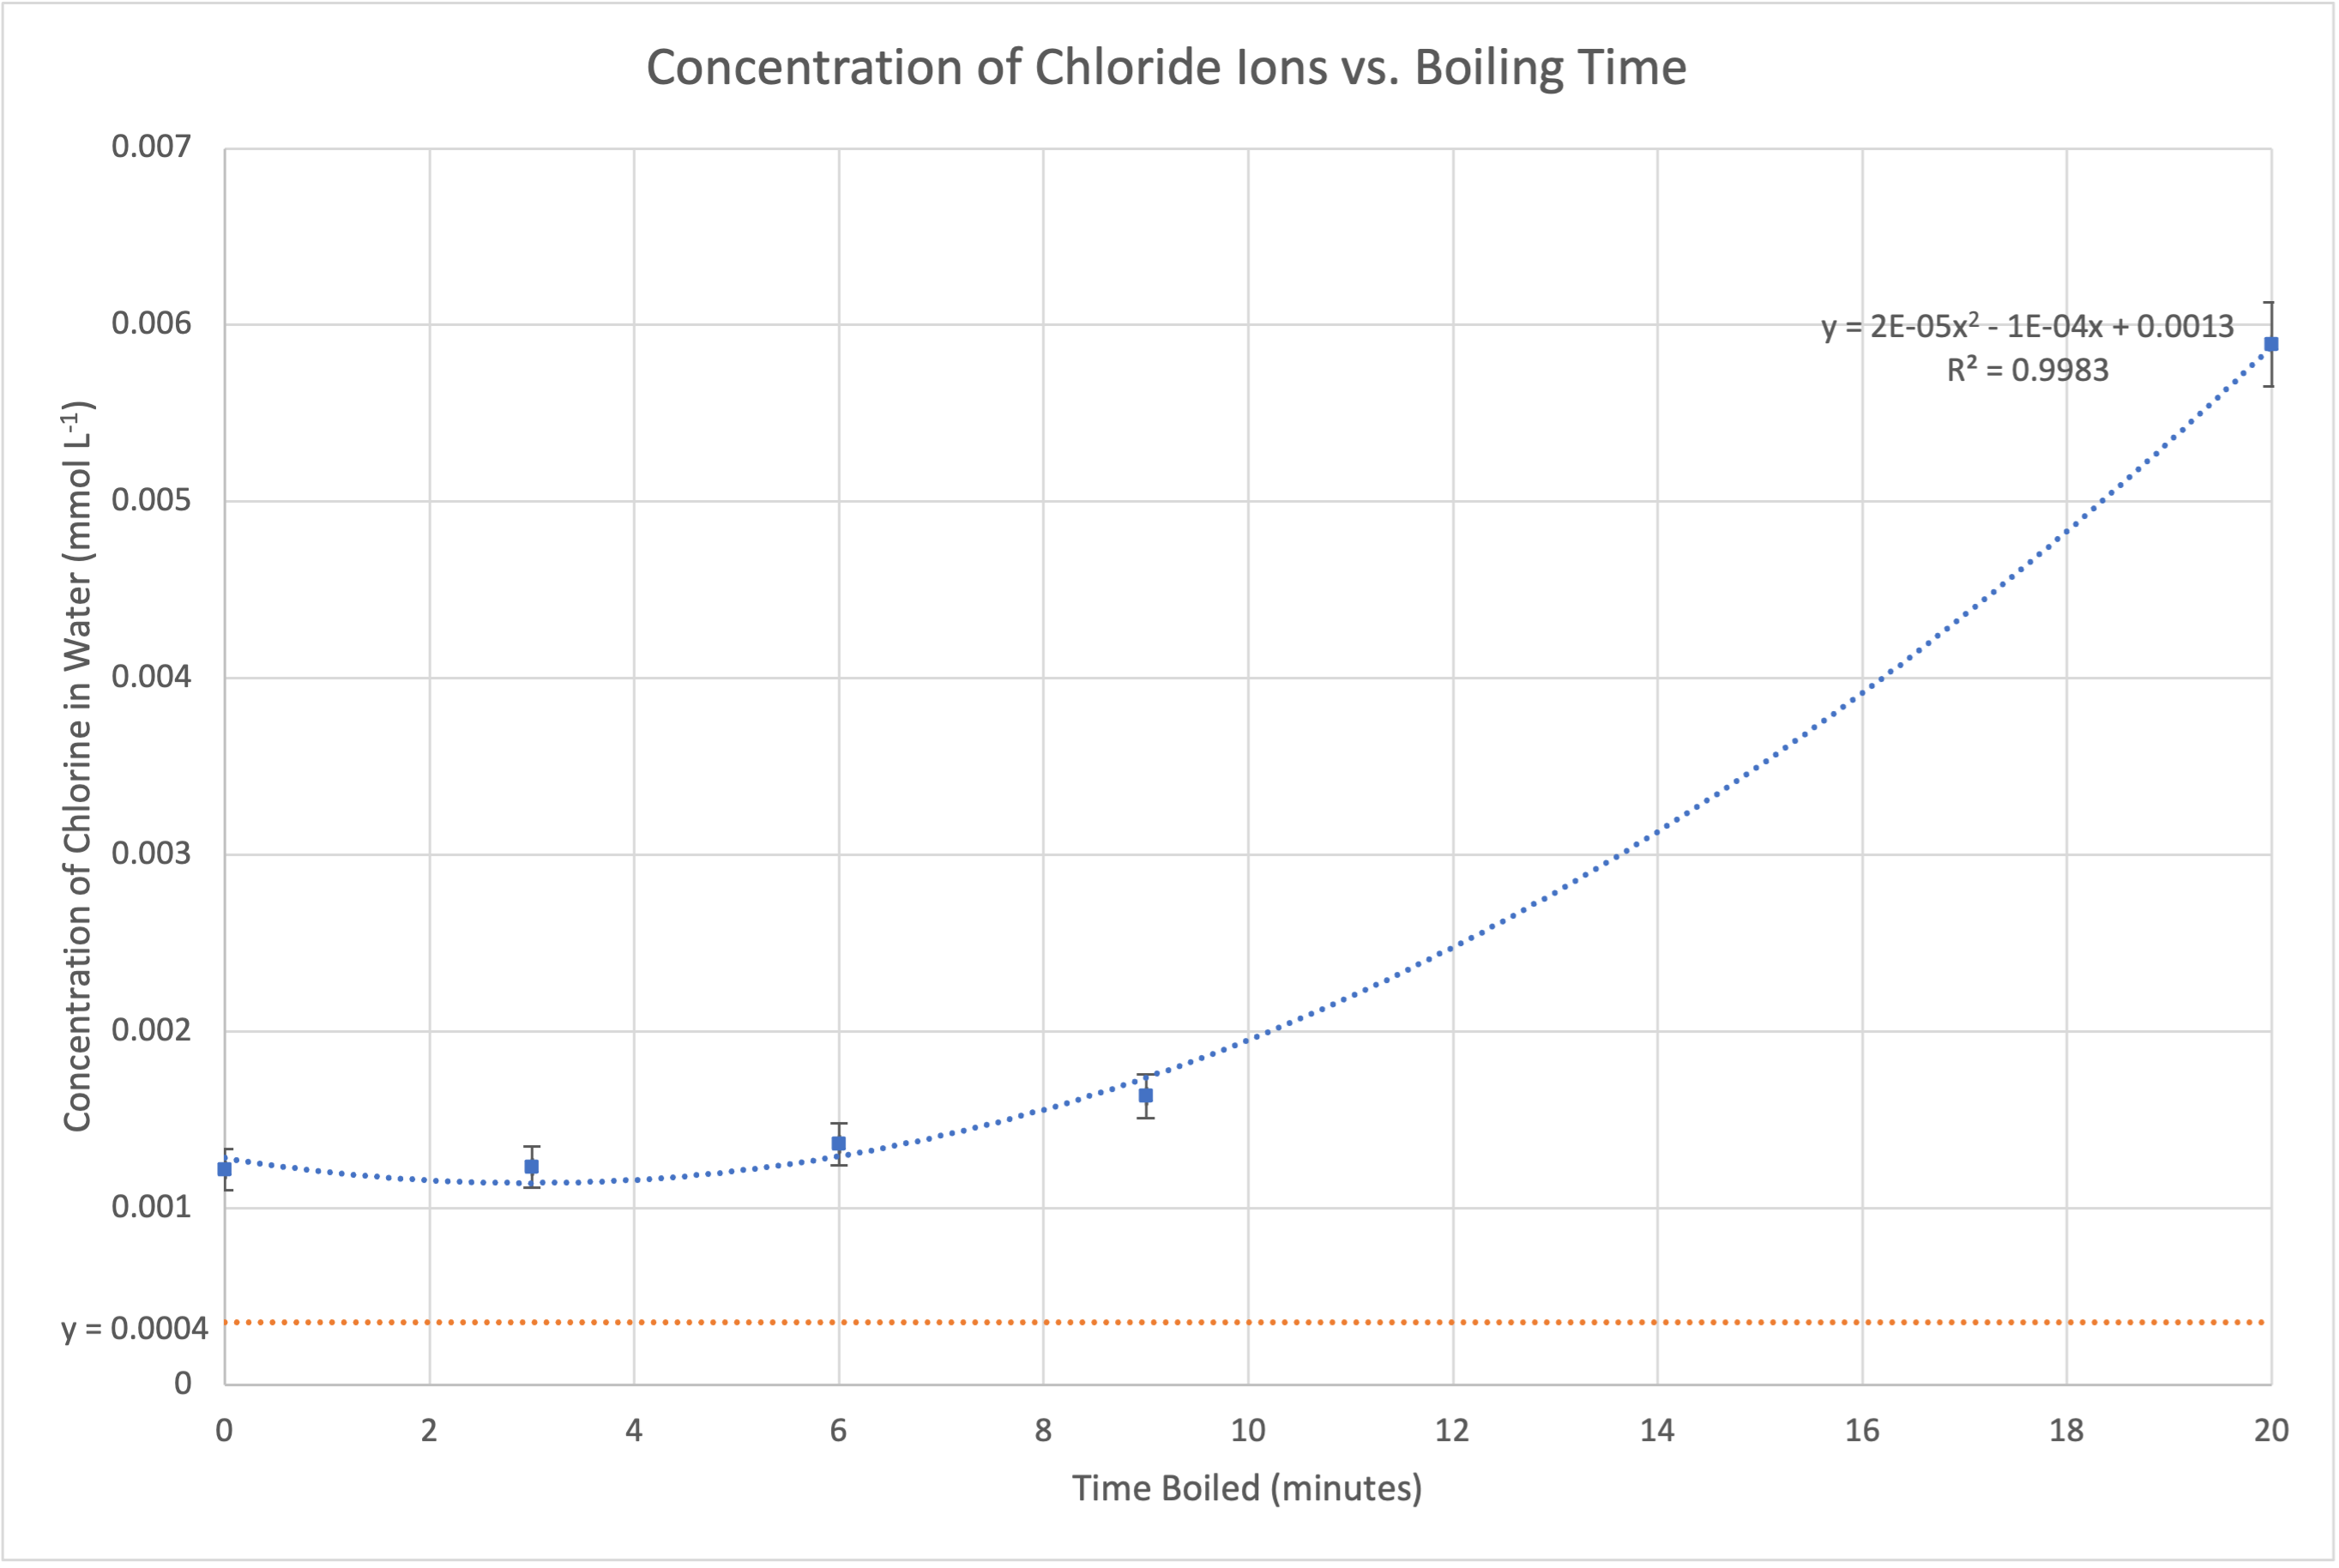
\includegraphics[width=\linewidth]{assets/concentration-vs-boiling-time.png}
\end{figure}

\section{Analysis}

\subsection{Identifying the Correlation}

The equation of the trendline can be written as follows, where $t$ represents the time the water has been boiled (in \si{\minute}) and $y$ represents the concentration of chloride in the water (in \si{\mmol}):
%
\begin{align*}
	y = 0.00002t^2 - 0.001t + 0.0013
\end{align*}

This equation indicates that there is a positive and quadratic relationship between boiling time and chlorine concentration. This relationship does not agree with the theory presented earler, where it was established that the chlorine concentration in the water should \textit{decrease} as the water was boiled for longer. Instead, the graph indicates that the chlorine concentration \textit{increases} as the water was boiled for longer.

\subsection{Explaining the Results}

During the research phase, two common methods of water disinfection were mentioned: disinfection with chlorine and disinfection with chloramine (\ce{NH2Cl}). The experiment was performed under the belief that Toronto used only chlorine instead of chloramine for water treatment.

However, after further investigation, it appears that there was a misunderstanding from one of the official sources. Contrary to initial beliefs, it was discovered that Toronto adds ammonia during their water treatment system as a secondary disinfectant (<?# todo: link source ?>). When ammonia is added to water with chlorine, the ammonia bonds to chlorine to produce chloramine (\ce{NH2Cl}). Compared to chlorine, chloramine is more stable because of the bond between chlorine and ammonia. This stability allows chloramine to remain in the water supply for a longer period of time to ensure that the water remains disinfected for longer. However, the extra stability of chloramine also makes boiling water an ineffective way to remove the excess chlorine in water (while it is possible to remove chloramine by boiling, it takes much longer than 20 minutes to remove an significant amount of chloramine).

Thus, based on the results presented in Figure 5 and the additional sources from further investigation, the water used in the experiment was likely treated with chloramine. This conclusion is further supported by the effectiveness of the deionizer used in trials 1 to 3, which removed significantly more chlorine than boiling water. Unlike boiling, the water deionizater is still effective at removing chloramine: the chloramine dissolves into positively charged ammonia ions and negatively changed chlorine ions in water, which are filtered out by the positive and negative resins in the water deionizer, respectively.

The increase in concentration in the graph can be attributed to the decrease in volume as water as the water was boiled for longer, while the amount of chloramine remained relatively the same. Since concentration is inversely proportional to the volume, when the volume decreases and the number of moles of chloramine are held constant, the concentration of chloramine increases.

<?# todo add equation ?>

The quadratic relationship is likely explained by the rate of evaporation as the water is boiled. Since chloramine is not effectively removed by boiling water, the only variable changing when the water is boiled is the remaining volume of water. As the volume of water decreases, the heat energy transferred to the water by the hot plate then heats up the water more quickly. Thus, as the water is boiling for longer, the amount of water that evaporates will increase over time, thus increasing the rate of concentration of chloramine in the water. % TODO: explain better e.g. with graph

Unfortunately, the final volume after boiling the samples of water was not recorded (due to the expectation that it would not be relevant to the experiment), limiting further analysis between the total amount of water remaining after boiling and the chloramine concentration in the water.

% TODO: cite https://www.toronto.ca/311/knowledgebase/kb/docs/articles/toronto-water/water-treatment-and-supply/water-treatment-plants/f.j.-horgan-treatment-plant/reasons-that-the-city-uses-chlorine-to-treat-drinking-water.html

\subsection{Comparison with Expected Value}

The accuracy of the titration can be determined by comparing the experimental results of chlorine concentration in unaltered tap water with the expected chlorine concentration regulated by the city of Toronto. Toronto's chlorine concentration is regulated to be between 1\mg/\litre and 3\mg/litre. In order to compare the experimental data with this value, the concentration of chlorine in \si{\mpl} must be converted to concentration in \si{\mg\per\litre}:
%
\begin{align*}
	m_{\ce{Cl^-}} & = n_{\ce{Cl^-}} \times M_{\ce{Cl^-}}
	\\
	M_{\ce{Cl^-}} & = 35.45\gpm
	\\
	m_{\ce{Cl^-}} & = <?= sf(trial1Calculations.molesOfChlorine, 3) ?> \pm 8.8\% \mmol \times 35.45\gpm
	\\
	<? trial1Calculations.massOfChlorine = trial1Calculations.molesOfSilverNitrate * 35.45 -?>
	m_{\ce{Cl^-}} & = <?= sf(trial1Calculations.massOfChlorine, 3) ?>\mg
\end{align*}

Converting this amount to \si{\mg\per\litre} gives us the following amount:
%
\begin{align*}
	c = <?= sf(trial1Calculations.massOfChlorine, 3) ?>\mg/10\ml
	\\
	c = <?= sf(trial1Calculations.massOfChlorine * 100, 3) ?>\mg/\litre
\end{align*}

This result is off by an order of magnitude: the experimental results indicate that there is over 10 times the amount of chlorine that is expected from Toronto's tap water. It is very unlikely that this discrepancy

\subsection{Potential Sources of Discrepancy}

The discrepancy between the experimental data and the expected data may be attributed to the dilute solutions of silver nitrate and potassium chromate used in the experiment. Due to availability limitations, the concentration of potassium chromate needed to be scaled down to 0.01\mpl compared to the recommend amount of 0.25\mpl to perform Mohr's titration. In addition, the concentration of silver nitrate solution needed to be scaled down to 0.01\mpl as well in order to gain more precision since the amount of tap water in chlorine is very trace. Thus, it is likely that the initial visual colour change was too faint to notice, and an excess of silver nitrate was needed in order to produce a visible colour change that indicated the titration's endpoint. However, this discrepancy would represent a systematic error in the experiment, and thus does not invalidate the positive correlation between the boiling time and the remaining chlorine concentration in water. % TODO: explain better

<?# TODO: add more possible reasons for this error ?>

\section{Conclusion}

While the results from this experiment may not have been accurate when compared to the expected amount of chlorine in Toronto's tap water, the data still displayed an evident trend between the amount of chlorine in water and the boiling time of water.

Despite the inaccuracy between the experimental value and the actual value, the strong positive correlation between boiling time and chlorine concentration strongly suggests that the city of Toronto uses chloramine to disinfect their water.

Thus, having learned that Toronto uses chloramine, my family should consider investing in a water filter or a reverse osmosis filter to remove the excess chlorine in water, which are more effective and efficient at removing chloramine than boiling.

\subsection{Future Improvements}



Since I didn't have access to a brand new carbon-based water filter or a reverse osmosis filter for this experiment, it would be interesting to compare their effectiveness at removing chloramine from water.

\end{document}

% TODO: add 1 strength and many weaknesses
% TODO: past passive

% TODO: **specific** improvements (e.g. a specific instrument)

% TODO: add theory, what would you do if you could increase the scope of the experiment

% TODO: add weakness of Mohr's method that there must be excess and no benzene or whatever